\begin{figure}[tb]
\centering
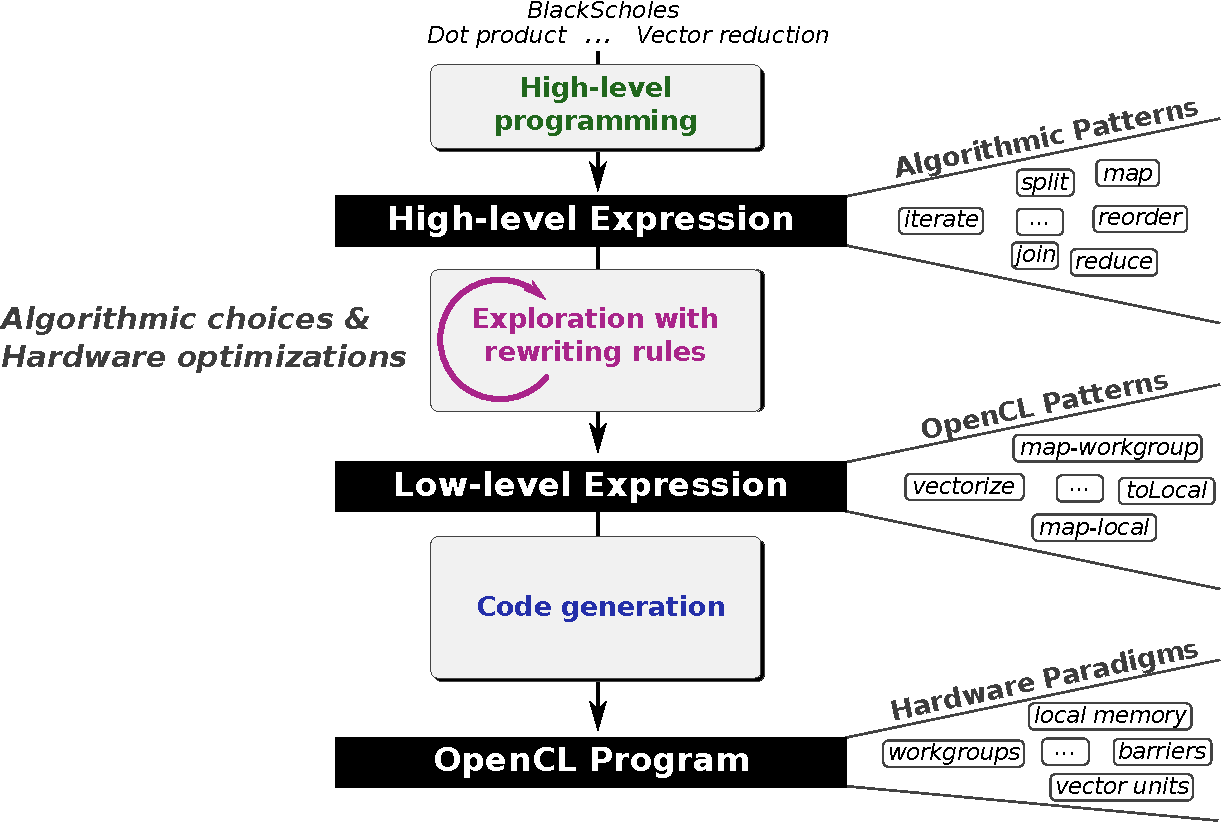
\includegraphics[width=\linewidth]{overviewPatternCodeGeneration}
\caption[Overview of our code generation approach.]{
Overview of our code generation approach.
Problems expressed with  high-level algorithmic patterns are systematically transformed into low-level \OpenCL patterns using a rule rewriting system.
% The application developer expresses the problem with high-level algorithmic patterns.
% These are systematically transformed into low-level \OpenCL patterns using a rule rewriting system.
\OpenCL code is generated by mapping the low-level patterns directly to the \OpenCL programming model representing hardware paradigms.
}
\label{fig:highlevel}
\end{figure}

\section{Overview of our Code Generation Approach}
\label{section:code-generation:overview}

The overview of our pattern-based code generation approach is presented in \autoref{fig:highlevel}.
The programmer writes a \emph{high-level expression} composed of \emph{algorithmic patterns}.
Using a rewrite rule system, we transform this high-level expression into a \emph{low-level expression} consisting of \emph{\OpenCL patterns}.
At this rewrite stage, algorithmic and optimization choices in the high-level expression are explored.
The generated low-level expression is then fed into our code generator that emits an \emph{\OpenCL program} which is, finally, compiled to machine code by the vendor-provided \OpenCL compiler.
A major advantage of our approach is that there is no analysis or optimizations performed in the code generator:
optimization decisions are made earlier in the rule rewrite system.
This results in a clear separation of concerns between the high-level patterns used by the programmer and the low-level hardware paradigms that enable performance portability.


\subsection{Introductory Example}

\begin{figure}[b]
\centering

\begin{subfigure}[b]{.85\linewidth}
\begin{lstlisting}[mathescape,numbers=left]
mul3 x     = x * 3    // user-defined function
vectorScal = map mul3          // map pattern
\end{lstlisting}
\caption{\textbf{High-level expression} written by the programmer.}
\label{fig:codeex:map}
\end{subfigure}

\begin{minipage}{0.1\linewidth}
\vspace{0pt}
\centering
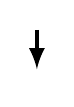
\begin{tikzpicture}[ultra thick]
 \draw [black,   -latex      ] (0,0.5) -- (0,0) node [] {};
\end{tikzpicture}
\end{minipage}
\begin{minipage}{0.25\linewidth}
\vspace{-5pt}
\centering
\textbf{rewrite rules}
\end{minipage}
\begin{minipage}{0.1\linewidth}
\vspace{0pt}
\centering
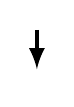
\begin{tikzpicture}[ultra thick]
 \draw [black,   -latex      ] (0,0.5) -- (0,0) node [] {};
\end{tikzpicture}
\end{minipage}

\begin{subfigure}[b]{\linewidth}
\centering
\begin{minipage}{.85\linewidth}%{0.85\textwidth}
\begin{lstlisting}[mathescape,numbers=left]
mul3 x     = x * 3
vectorScal = join $\circ$ map-workgroup ($\label{fig:codeex:impl:map-wg}$
                    asScalar $\circ$ map-local ($\label{fig:codeex:impl:map-wg:start}$
                      vect 4 mul3$\label{fig:codeex:impl:vec}$
                    ) $\circ$ asVector 4$\label{fig:codeex:impl:map-wg:stop}$$\label{fig:codeex:impl:asVec}$
                 ) $\circ$ split 1024
\end{lstlisting}
\end{minipage}
\caption{\textbf{Low-level expression} derived using rewrite rules.}
\label{fig:codeex:impl}
\end{subfigure}

\begin{minipage}{0.1\linewidth}
\vspace{0pt}
\centering
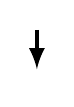
\begin{tikzpicture}[ultra thick]
 \draw [black,   -latex      ] (0,0.5) -- (0,0) node [] {};
\end{tikzpicture}
\end{minipage}
\begin{minipage}{0.26\linewidth}
\vspace{-5pt}
\centering
\textbf{code generator}
\end{minipage}
\begin{minipage}{0.1\linewidth}
\vspace{0pt}
\centering
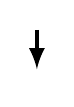
\begin{tikzpicture}[ultra thick]
 \draw [black,   -latex      ] (0,0.5) -- (0,0) node [] {};
\end{tikzpicture}
\end{minipage}

\begin{subfigure}[b]{\linewidth}
\centering
\begin{minipage}{.85\textwidth}
\begin{lstlisting}[mathescape,numbers=left]
float4 mul3(float4 x) { return x * 3; }$\label{fig:codeex:ocl:def}$

kernel vectorScal(global float* in,
                  global float* out, int len) {
 for (int i =get_group_id(0); i < len/1024;$\label{fig:codeex:ocl:loop1:start}$
          i+=get_num_groups(0)) {$\label{fig:codeex:ocl:loop1:end}$
  global float* grp_in  = in+(i*1024);
  global float* grp_out = out+(i*1024);
  for (int j =get_local_id(0); j < 1024/4;$\label{fig:codeex:ocl:loop2:start}$
           j+=get_local_size(0)) {$\label{fig:codeex:ocl:loop2:end}$
    global float4* in_vec4 =(float4*)grp_in+(j*4);
    global float4* out_vec4=(float4*)grp_out+(j*4);
    *out_vec4 = mul3(*in_vec4);$\label{fig:codeex:ocl:call}$
} } }  
\end{lstlisting}
\end{minipage}
\caption{\textbf{\OpenCL program} produced by our code generator.}
\label{fig:codeex:ocl}
\end{subfigure}
\caption[Introductory example: vector scaling.]{
Pseudo-code representing vector scaling.
The user maps the \code{mul3} function over the input array~(\subref{fig:codeex:map}).
This high-level expression is transformed into a low-level expression~(\subref{fig:codeex:impl}) using rewrite rules.
Finally, our code generator turns the low-level expression into an \OpenCL program~(\subref{fig:codeex:ocl}).
}
  \label{fig:codeex}
\end{figure}

We illustrate the advantages of our approach using a simple vector scaling example shown in \autoref{fig:codeex} on page \pageref{fig:codeex}.
The user expresses the computation by writing a high-level expression using the algorithmic \pat{map} pattern as shown in \autoref{fig:codeex:map}.
This coding style is similar to functional programming as we saw with the \SkelCL programming model introduced in \autoref{chapter:skelcl}.
As common in functional programming, the $\circ$ operator represents sequential function composition. %, \ie, $(f \circ g)\ x = f(g\ x)$.

Our technique first rewrites the high-level expression into a representation closer to the \OpenCL programming model.
This is achieved by applying rewrite rules which are presented later in \autoref{section:rules}.
\autoref{fig:codeex:impl} shows one possible derivation of the original high-level expression.
Other derivations are possible with different optimizations applied.
The particular expression shown in \autoref{fig:codeex:impl} features vectorization as one possible optimization technique.
In the derived low-level expression, starting from the last line, the input is split into chunks of a fixed number of elements, 1024 in the example.
Each chunk is then mapped onto an \OpenCL work-group with the \pat{map-workgroup} low-level pattern (\autoref{fig:codeex:impl:map-wg}).
Within a work-group (\autoref{fig:codeex:impl:map-wg:start}---\autoref{fig:codeex:impl:map-wg:stop}), we vectorize the elements (\autoref{fig:codeex:impl:asVec}), each mapped to a local work-item inside a work-group via the \pat{map-local} pattern (\autoref{fig:codeex:impl:map-wg:start}).
Each local work-item now processes 4 elements, enclosed in a vector type.
Finally, the \pat{vect-4} pattern (\autoref{fig:codeex:impl:vec}) vectorizes the user-defined function \code{mul3}.
The exact meaning of our patterns will be given in \autoref{section:patterns}.

The last step consists of traversing the low-level expression and generating \OpenCL code for each low-level pattern encountered (\autoref{fig:codeex:ocl}).
Each map patterns generates a for-loop (\autoref{fig:codeex:ocl:loop1:start}---\autoref{fig:codeex:ocl:loop1:end} and \autoref{fig:codeex:ocl:loop2:start}---\autoref{fig:codeex:ocl:loop2:end}) that iterate over the input array assigning work to the work-groups and local work-items.
The information of how many chunks each work-group and work-items processes comes from the corresponding \pat{split}.
In \autoref{fig:codeex:ocl:call} the vectorized version of the user-defined \code{mul3} function (defined in \autoref{fig:codeex:ocl:def}) is applied to the input array.

To summarize, our approach consists of generating \OpenCL code starting from a single portable high-level program representation of a program.
This is achieved by systematically transforming the high-level expression into a low-level form suitable for code generation.
The next three sections present our high-level and low-level patterns, the rewrite rules, and the code generation mechanism.

